% !TEX root = ../main.tex

\subsection{ATLAS Humanoid Robot}

\ldots

\begin{figure}[t]
\centering
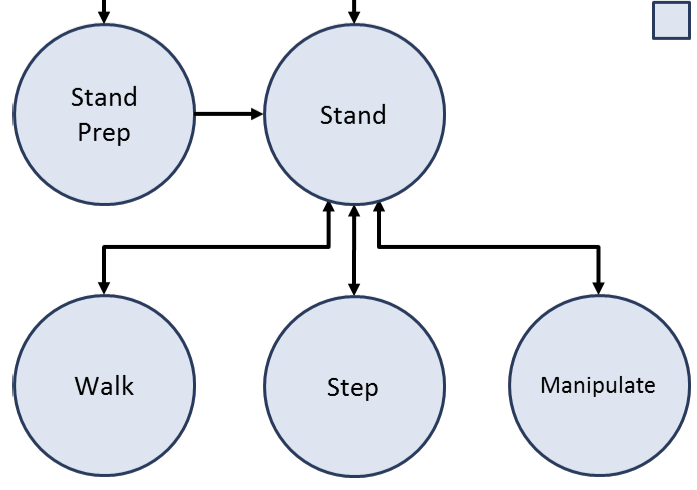
\includegraphics[width=0.99\columnwidth,clip]{./img/control_modes_ts.png}
\caption{
	\todo[inline, caption = {Create a simple control mode TS figure}]{Placeholder! Create simple control mode TS figure (flat).}
}
\label{Fig:ControlModeTS}
%\vspace{-3 pt}
\end{figure}

\subsection{Team ViGIR's Approach to High-level Control}

\ldots FlexBE\footnote{\scriptsize{\url{https://github.com/team-vigir/flexbe_behavior_engine}}}
, GUI\footnote{\scriptsize{\url{https://github.com/team-vigir/flexbe_chrome_app}}}
, behaviors and states\footnote{\scriptsize{\url{https://github.com/team-vigir/vigir_behaviors}}}.

\begin{figure}[t]
\centering
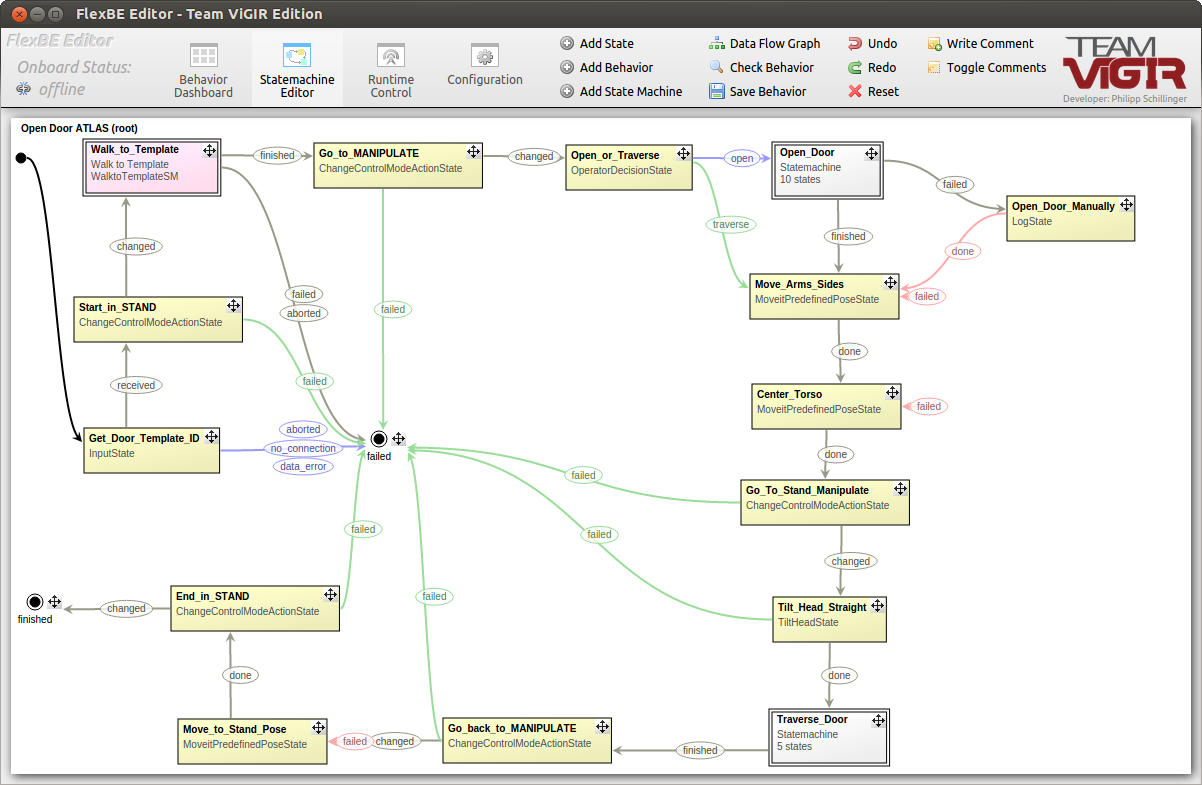
\includegraphics[width=0.99\columnwidth,clip]{./img/behavior_open_door.png}
\caption{A high-level behavior for carrying out the DRC Finals' ``Door" task.
It was designed by Team ViGIR developers using the FlexBE Editor (graphical user interface).
}
\label{Fig:FlexBESM}
\end{figure}

\subsection{Linear Temporal Logic and Reactive LTL Synthesis}

\ldots